
\documentclass[dvipdfmx]{standalone}
\usepackage[T1]{fontenc}
\usepackage{newtxtext, newtxmath}

\usepackage{tikz}
\usetikzlibrary{shapes.multipart}
\usetikzlibrary{shapes.arrows}
\usetikzlibrary{calc, positioning}

\begin{document}
  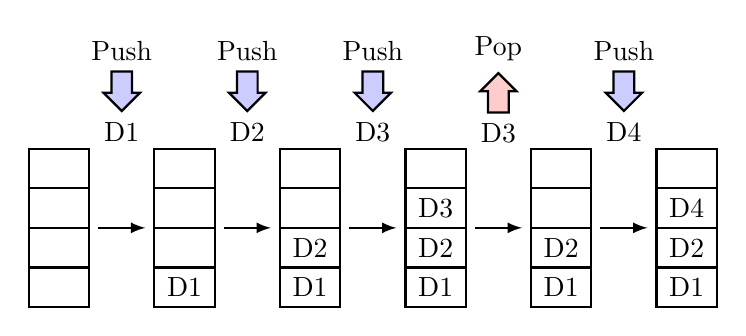
\begin{tikzpicture}[thick, > = latex, shorten > = 1mm, shorten < = 1mm]
    \tikzset{
      my rectangle split/.style={
        rectangle split, rectangle split parts=#1, draw, anchor=center,
        rectangle split ignore empty parts=false
      },
      my data arrow/.style={
        draw, single arrow, minimum height=5mm, single arrow head extend=1mm,
      },
    }
    % Draw stacks
    \def\EmptyCell{\phantom{DN}}
    \node (stack1) [my rectangle split=4]
    {\EmptyCell \nodepart{two} \EmptyCell \nodepart{three} \EmptyCell \nodepart{four} \EmptyCell};
    \node (stack2) [my rectangle split=4, right=8mm of stack1]
    {\EmptyCell \nodepart{two} \EmptyCell \nodepart{three} \EmptyCell \nodepart{four} D1};
    \node (stack3) [my rectangle split=4, right=8mm of stack2]
    {\EmptyCell \nodepart{two} \EmptyCell \nodepart{three} D2 \nodepart{four} D1};
    \node (stack4) [my rectangle split=4, right=8mm of stack3]
    {\EmptyCell \nodepart{two} D3 \nodepart{three} D2 \nodepart{four} D1};
    \node (stack5) [my rectangle split=4, right=8mm of stack4]
    {\EmptyCell \nodepart{two} \EmptyCell \nodepart{three} D2 \nodepart{four} D1};
    \node (stack6) [my rectangle split=4, right=8mm of stack5]
    {\EmptyCell \nodepart{two} D4 \nodepart{three} D2 \nodepart{four} D1};

    % Arrows
    \foreach[count=\i, count=\n from 2] \data\rotate in {D1/270, D2/270, D3/270, D3/90, D4/270} {
      \draw[->] (stack\i) -- (stack\n) node[midway] (stack\i-\n) {};
      \ifnum\rotate=90
        % Pop
        \draw (stack\i-\n) +(up:1.65cm)
          node (process\i) [my data arrow, shape border rotate=\rotate, fill=red!20] {};
        \draw (process\i.tip) node[above] {Pop};
        \draw (process\i.tail) node[below] {\data};
      \else
        % Push
        \draw (stack\i-\n) +(up:1.8cm)
          node (process\i) [my data arrow, shape border rotate=\rotate, fill=blue!20] {};
        \draw (process\i.tail) node[above] {Push};
        \draw (process\i.tip) node[below] {\data};
      \fi
    }

  \end{tikzpicture}
\end{document}
